\documentclass{sintefbeamer}

% packages, font, color, and newcommands
\usepackage{amsfonts, amsmath, oldgerm, lmodern, bm}
% \usepackage[font={footnotesize}]{caption}
\usepackage{natbib}
\bibliographystyle{apalike}
\usefonttheme{serif}

\title{A phenomenological description of pairwise interactions in emulsion.}
\subtitle{Based on numerical simulations results.}
\author{\href{http://basilisk.fr/sandbox/fintzin/Rising-Suspenion/RS.c}{\underline{N. Fintzi}, JL. Pireson and S. Popinet. }}
% \date{Created on May 22, 2022}

\titlebackground{image/3D/PHI01.png}

% document body

\newcommand{\size}{0.22\textwidth}
\newcommand{\avg}[1]{\left<#1\right>}
\newcommand{\davg}[1]{\left<#1\right>_d}
\newcommand{\cavg}[1]{\left<#1\right>_c}
\newcommand{\kavg}[1]{\left<#1\right>_k}
\newcommand{\Iavg}[1]{\left<#1\right>_I}
\newcommand{\pavg}[1]{n \left<#1\right>_p}
\newcommand{\pnavg}[1]{\left<#1\right>_p}
% \newcommand{\nstavg}[1]{\left<#1\right>_{nst}}
\newcommand{\nstavg}[1]{\overline{#1}_{nst}}
\newcommand{\mavg}[1]{\left<#1\right>_m}
\newcommand{\lavg}[1]{\theta_0\left<#1\right>^\lambda}
\newcommand{\partials}[1]{\partial_{i_1}\partial_{i_2}\ldots\partial{i_{#1}}}
\newcommand{\partialp}[2]{ \prod_{m=#1}^{#2} \partial_{i_m}}
\newcommand{\hatpartialp}[2]{ \prod_{m=#1}^{#2} \hat{\partial}_{j_m}}
\newcommand{\hatpartialpi}[2]{ \prod_{m=#1}^{#2} \hat{\partial}_{i_m}}
\newcommand{\pri}[2]{ \prod_{m=#1}^{#2} r_{i_m}}
\newcommand{\prj}[2]{ \prod_{m=#1}^{#2} r_{j_m}}
\newcommand{\nablab}{\bm{\nabla}}
\newcommand{\nablabh}{\hat{\bm{\nabla}}}
\newcommand{\ddt}{\frac{d}{d t}}
\newcommand{\pddt}{\frac{\partial}{\partial t}}


\begin{document}
\maketitle
\section{Theoretical background on the kinetic theory}

\begin{frame}{Kinetic theory or Population Balance Equation (PBE) to describe poly-disperse multiphase flows.}
  \begin{definition}
    \begin{itemize}
      \item Let $\mathcal{F}^N$ be a configuration of $N$ particles in the dispersed phase (where $N$ is the maximum number of particles in the flow).  
      \item Then $\mathcal{F}^N = \left\{\textbf{x}^1,\textbf{u}^1\ldots \textbf{x}^N,\textbf{u}^N\right\}$, is the vector containing all parameters of the dispersed phase such as the velocity the position and all other properties of each particle.  
      \item $P(\mathcal{F}^N,t)$ is the probability density of having the dispersed phase in the state $\mathcal{F}^N$, at time $t$. 
    \end{itemize}
  \end{definition}

  Transport equation of the Probability Density Function (PDF) :

  \begin{equation*}
    \pddt P(\mathcal{F}^N,t) 
    + \frac{\partial}{\partial \mathcal{F}^N} \cdot \left(
      \frac{\partial \mathcal{F}^N}{\partial t} P(\mathcal{F}^N,t)
    \right)
    = S(\mathcal{F}^N,t) 
  \end{equation*}
  \begin{itemize}
    \item $S(t)$ is a source term due to interaction between particles, such as break-up coalesce and collisions phenomenons. 
  \end{itemize}
\end{frame}

\begin{frame}{Modeling of the source term $S$}
  If we consider solely coalesce events, $S(\mathcal{F}^N,t)$ can be modeled by,
  \begin{equation*}
    S(\mathcal{F}^1,\mathcal{F}^2,t) 
    =  P^{(2)}(\mathcal{F}^{1},\mathcal{F}^{2},t) (\textbf{u}^1 - \textbf{u}^2)\cdot (\textbf{x}^1 - \textbf{x}^2) 
  \end{equation*} 
$P^2(\mathcal{F}^1,\mathcal{F}^2 ,t)$ is the \textbf{reduced} PDF of finding two particles in the flow, with the states $\mathcal{F}^1$ and $\mathcal{F}^2$ at time $t$. 
It is defined such as, 
  $$P^2(\mathcal{F}^1,\mathcal{F}^2 ,t) = \int P(\mathcal{F}^N ,t) d\mathcal{F}^{N-2}$$.
\begin{itemize}
  \item This model implies to know a priori, the relative velocities and positions distribution of each pairs of particles. 
\end{itemize}
\end{frame}

\begin{frame}
  \frametitle{The nearest particle statistics.}
In instead of using the reduced \textbf{pair} PDF, $P^2$, 
% \begin{equation*}
%   P^{(2)}(\mathcal{F}^1,\mathcal{F}^2 ,t) = \int P(\mathcal{F}^N,t) d\mathcal{F}^{N-2},
% \end{equation*}
we propose instead, to use the \textbf{nearest} PDF, as a droplet will coalesce solely with its nearest neighbor.
It reads,
\begin{equation*}
  P_{nst}(\mathcal{F}^1,\mathcal{F}^2 ,t) = \int h(\textbf{x}^1, \textbf{x}^2) P(\mathcal{F}^N,t) d\mathcal{F}^{N-2},
\end{equation*}
where $h=1$, if $\textbf{x}^1, \textbf{x}^2$ are the closest vector from the set of all position of $\mathcal{F}$, otherwise $h=0$. 
If $q$ is an arbitrary quantity linked to a particle, then, 
$$\nstavg{q}(\mathcal{F}^1,\mathcal{F}^2 ,t) =\frac{1}{P_{nst}} \int q(\mathcal{F}^2,t) h(\textbf{x}^1, \textbf{x}^2) P(\mathcal{F}^N,t) d\mathcal{F}^{N-2}$$,
is the averaged of the quantity $q$ on all pair of particles in the state $\mathcal{F}^1$ and $\mathcal{F}^2$, knowing that the particle $1$ is the closest neighbor of $2$. 
\end{frame}
\begin{frame}
  \frametitle{Conditional PDF}
  And, $P_{nst}(\mathcal{F}^1| \mathcal{F}^2, t)$ is the probability of having a Particle in the state $\mathcal{F}^2$ knowing that a particle is in the state $\mathcal{F}^2$ and that this particle is the closet from the former. 
  We now assume that $\mathcal{F}$ contain uniquely all vector of position \textbf{x}. 
  Then the probability that a particle is at the position $\textbf{x}^2$ knowing its nearest neighbor at $\textbf{x}^1$ can be obtained by,
  \begin{equation*}
    P_{nst}(\textbf{r})=P_{nst}(\textbf{x}^2 | \textbf{x}^1 , t) = \frac{P_{nst}(\textbf{x}^1,\textbf{x}^2)}{P(\textbf{x}^1)},
  \end{equation*} 
  where $\textbf{r} = \textbf{x}^2 - \textbf{x}^1$.
  Similarly, the fields of a quantity $q$ conditional on the presence of a particle at $\textbf{x}^1$ is obtained by, 
  \begin{equation*}
    \nstavg{q}(\textbf{r}) =\nstavg{q}(\textbf{x}^2 | \textbf{x}^1 , t) = \frac{\nstavg{q}(\textbf{x}^1,\textbf{x}^2 ,t)}{P(\textbf{x}^1)}.
  \end{equation*}


\end{frame}


\section{Visual insight of particles interactions}
\begin{frame}
\frametitle{Discrete probability density function for data treatment}


3D numerical simulation were performed in the range : 
\begin{itemize}
  \item The \textit{Galileo} number : $Ga = [5, 100]$
  \item The \textit{Bond} number : $Bo = 1$ (neaely spherical droplets)
  \item The volume fraction of dispersed phase : $\phi = [0.02;0.15]$. 
  \item The density and viscosity ratio, $\mu_r=\rho_r=1$. 
\end{itemize}

\underline{Show a video of a typical simulation}



\end{frame}
\begin{frame}
  \frametitle{From isotropic to oriented flows}

  \begin{figure}
    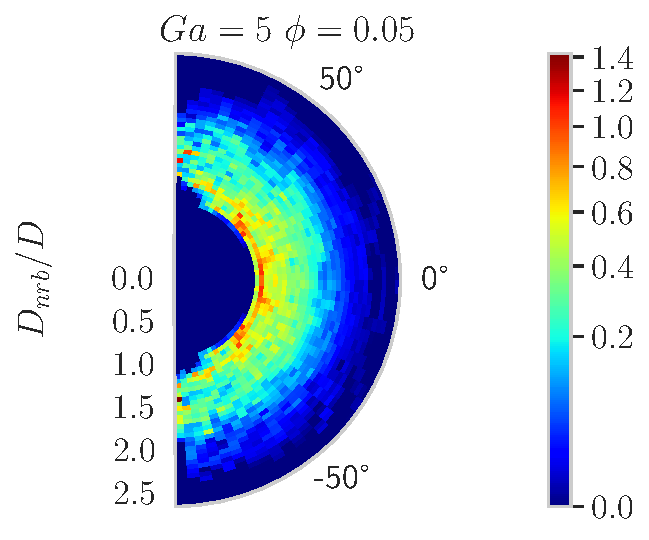
\includegraphics[height=0.15\textwidth]{image/Dim_3/fDrop/Dmin_Theta_Ga_5_PHI_0_05.pdf}
    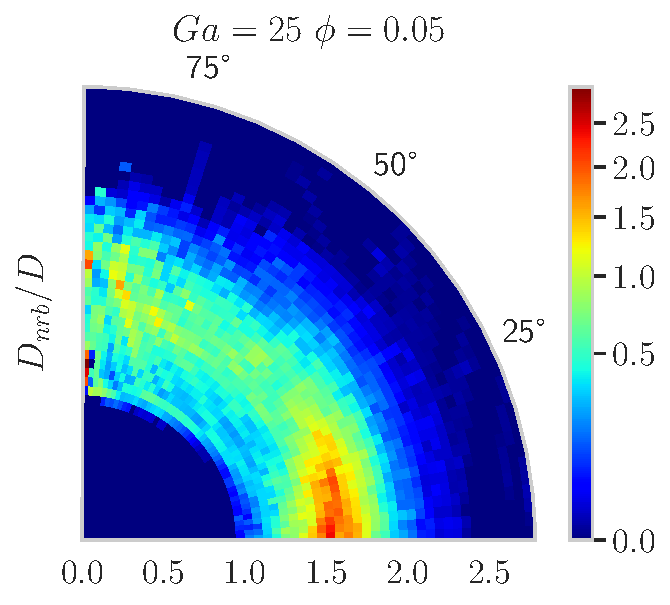
\includegraphics[height=0.15\textwidth]{image/Dim_3/fDrop/Dmin_Theta_Ga_25_PHI_0_05.pdf}
    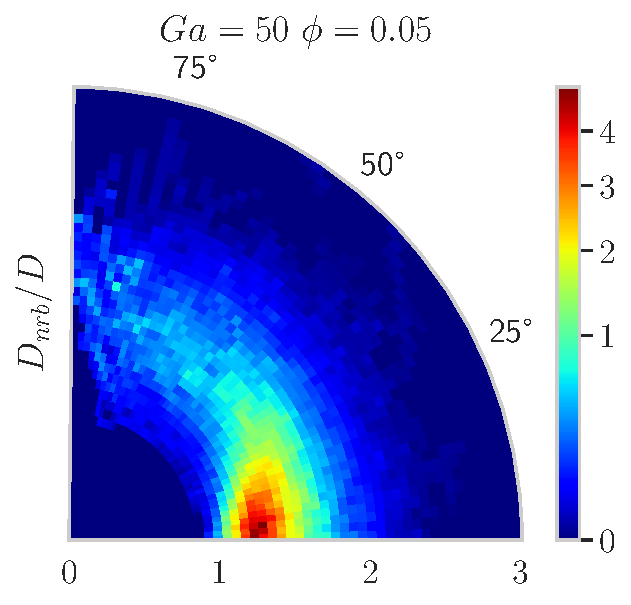
\includegraphics[height=0.15\textwidth]{image/Dim_3/fDrop/Dmin_Theta_Ga_50_PHI_0_05.pdf}
    
    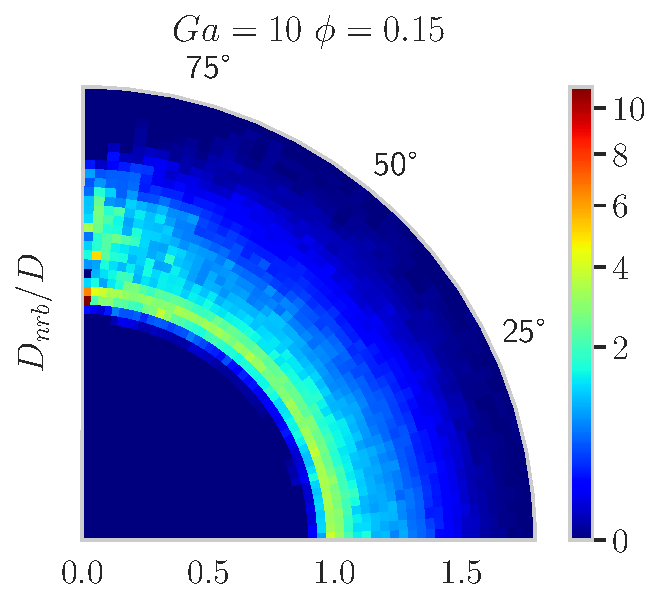
\includegraphics[height=0.15\textwidth]{image/Dim_3/fDrop/Dmin_Theta_Ga_10_PHI_0_15.pdf}
    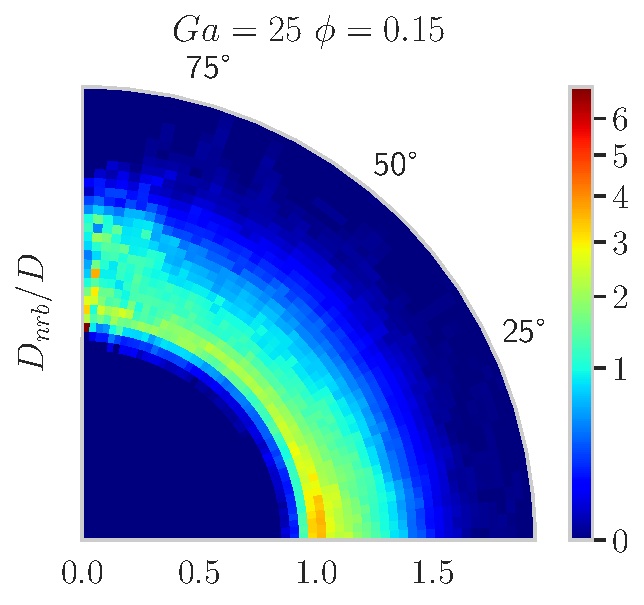
\includegraphics[height=0.15\textwidth]{image/Dim_3/fDrop/Dmin_Theta_Ga_25_PHI_0_15.pdf}
    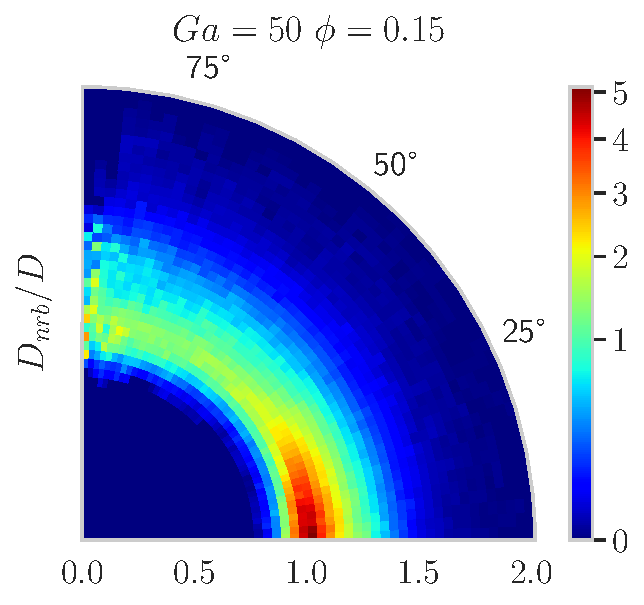
\includegraphics[height=0.15\textwidth]{image/Dim_3/fDrop/Dmin_Theta_Ga_50_PHI_0_15.pdf}
    \caption{Plots of $P_{nst} (\textbf{r})$ for different $Ga$ and $\phi$}
  \end{figure}

\begin{itemize}
  \item A preferred orientation is clearly visible for low $\phi$ and high $Ga$. 
  \item It is a direct representation of the Drafting -Kissing tumbling mechanism. 
\end{itemize}
\end{frame}

\begin{frame}
  \frametitle{Reconstruction of the nearest relative velocity fields}

  \begin{figure}
    % 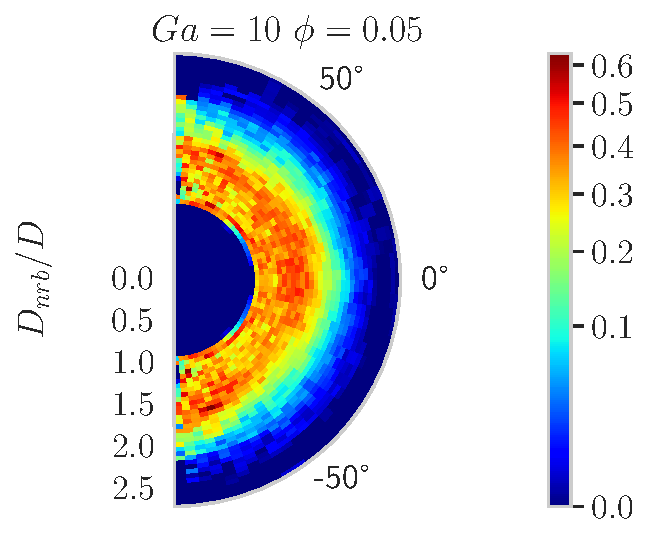
\includegraphics[height=0.15\textwidth]{image/Dim_3/fDrop/Dmin_Theta_Ga_10_PHI_0_05.pdf}
    % 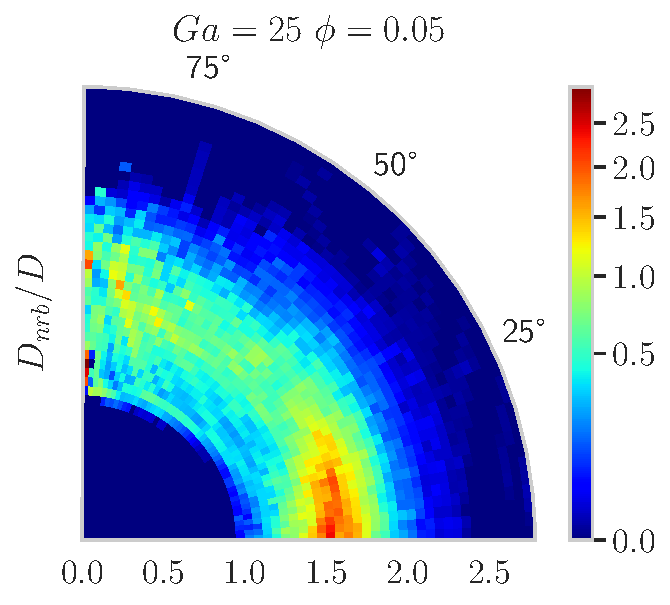
\includegraphics[height=0.15\textwidth]{image/Dim_3/fDrop/Dmin_Theta_Ga_25_PHI_0_05.pdf}
    % 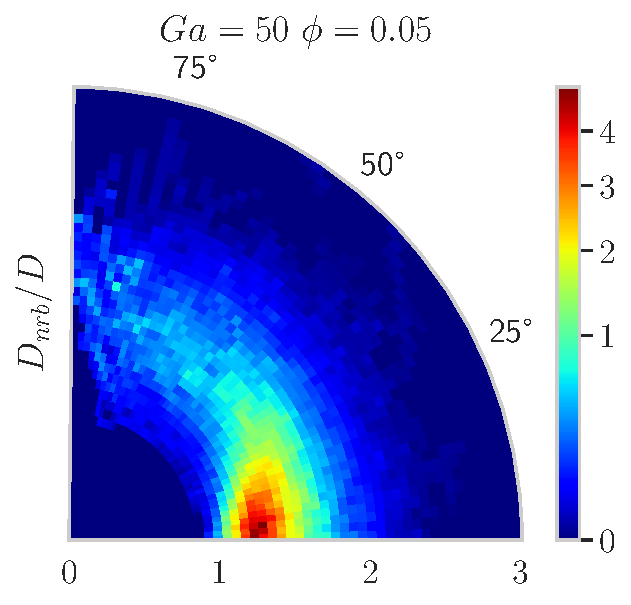
\includegraphics[height=0.15\textwidth]{image/Dim_3/fDrop/Dmin_Theta_Ga_50_PHI_0_05.pdf}

    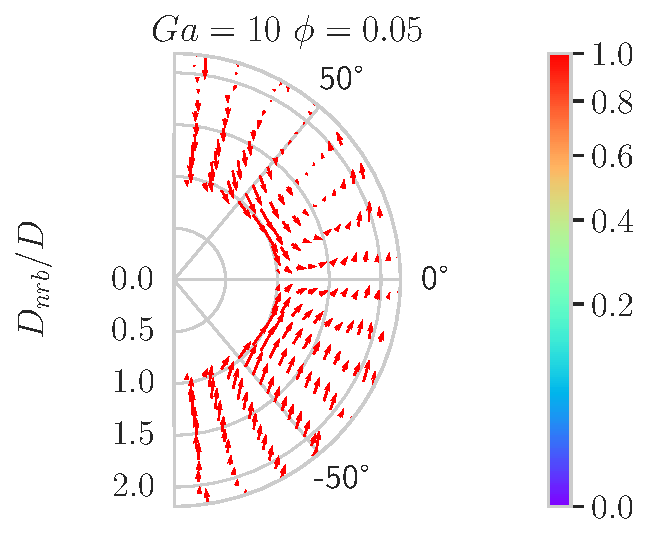
\includegraphics[height=0.2\textwidth]{image/Dim_3/fDrop/Dmin_Theta_U_rel_Ga_10_PHI_0_05.pdf}
    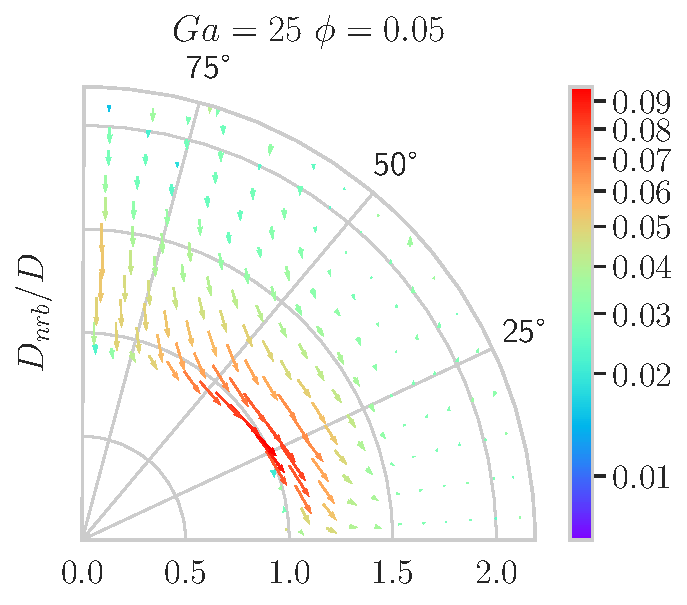
\includegraphics[height=0.2\textwidth]{image/Dim_3/fDrop/Dmin_Theta_U_rel_Ga_25_PHI_0_05.pdf}
    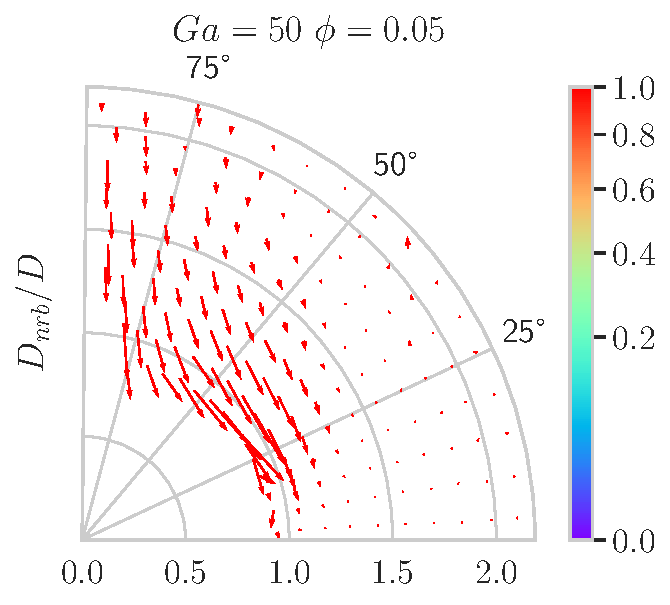
\includegraphics[height=0.2\textwidth]{image/Dim_3/fDrop/Dmin_Theta_U_rel_Ga_50_PHI_0_05.pdf}
    
    \caption{Nearest averaged velocity fields, $\nstavg{\textbf{u}} (\textbf{r})$ for different $Ga$ and $\phi$. The color map scale the magnitude of the relative velocity $|\textbf{u}^2 - \textbf{u}^1|$. }
  \end{figure}

\begin{itemize}
  \item Particles approach from the top and leave through the sides. 
  \item It is, again, a direct representation of the Drafting -Kissing tumbling mechanism since the velocity fields converge toward high density zone. 
\end{itemize}
\end{frame}

\begin{frame}
  \frametitle{Energy exchange during interaction}

  \begin{figure}
    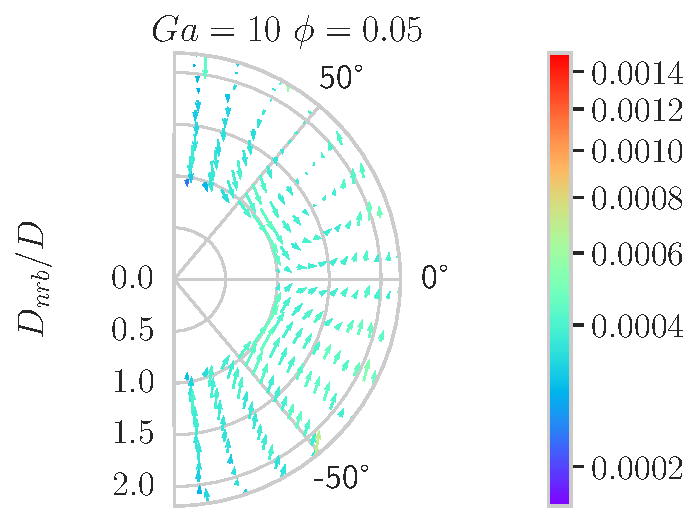
\includegraphics[height=0.2\textwidth]{image/Dim_3/fDrop/Dmin_Theta_Ec_Ga_10_PHI_0_05.pdf}
    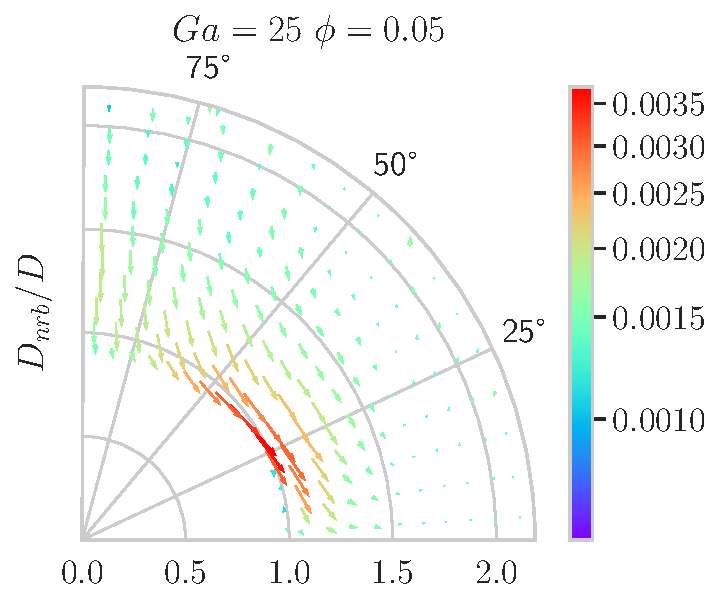
\includegraphics[height=0.2\textwidth]{image/Dim_3/fDrop/Dmin_Theta_Ec_Ga_25_PHI_0_05.pdf}
    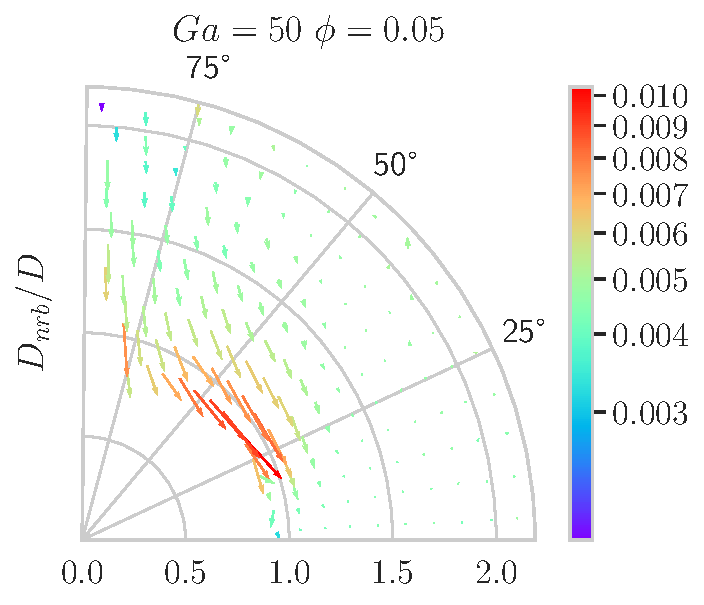
\includegraphics[height=0.2\textwidth]{image/Dim_3/fDrop/Dmin_Theta_Ec_Ga_50_PHI_0_05.pdf}

    % 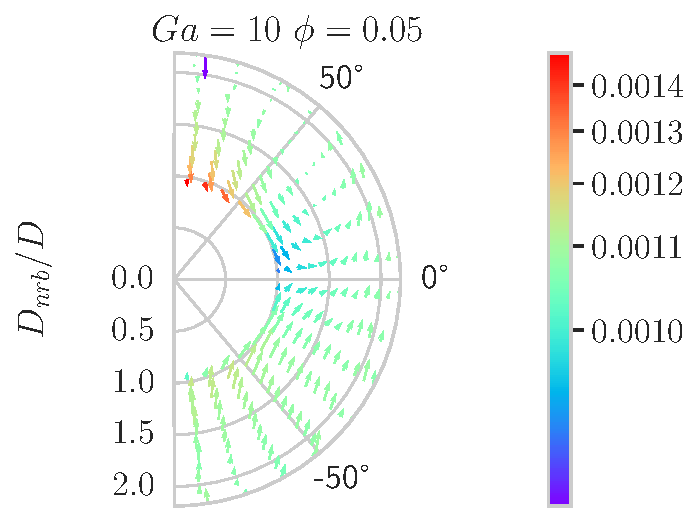
\includegraphics[height=0.2\textwidth]{image/Dim_3/fDrop/Dmin_Theta_ed_nbr_Ga_10_PHI_0_05.pdf}
    % 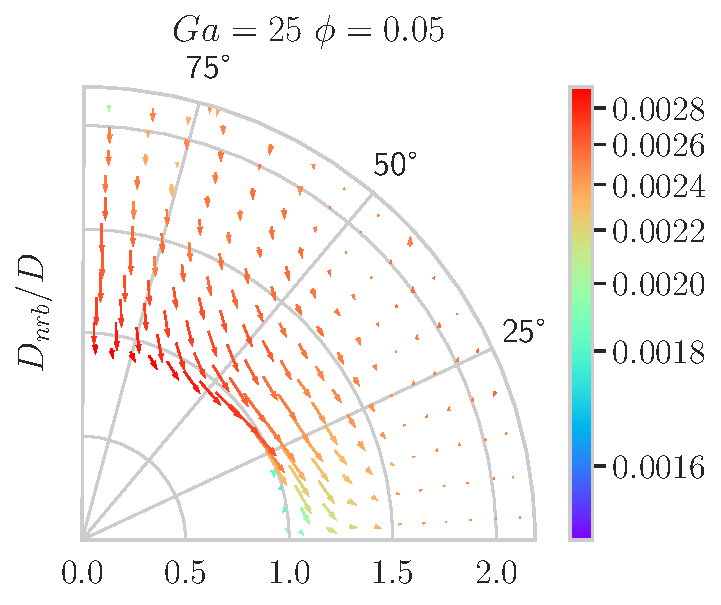
\includegraphics[height=0.2\textwidth]{image/Dim_3/fDrop/Dmin_Theta_ed_nbr_Ga_25_PHI_0_05.pdf}
    % 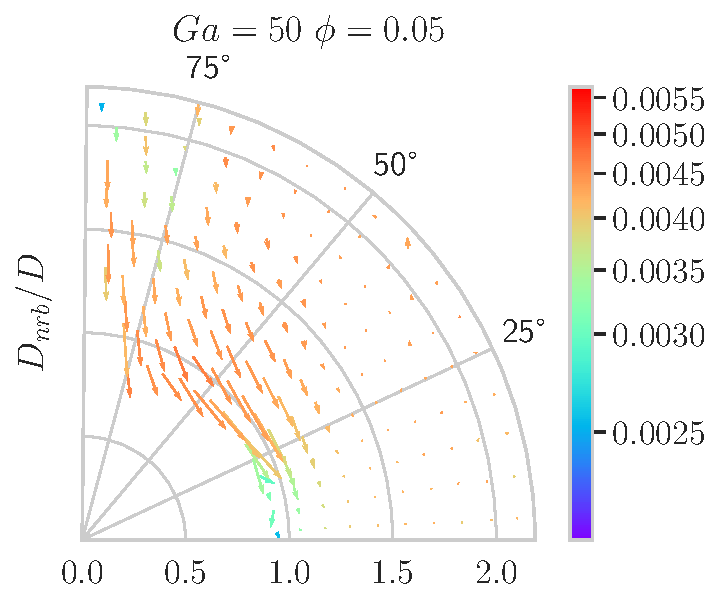
\includegraphics[height=0.2\textwidth]{image/Dim_3/fDrop/Dmin_Theta_ed_nbr_Ga_50_PHI_0_05.pdf}
    
    \caption{Nearest averaged velocity fields, $\nstavg{\textbf{u}}(\textbf{r})$ for different $Ga$ and $\phi$. 
    The color map scale, the relative kinetic Energy, i.e.  $\nstavg{E_c^1 - E_c^2}$.}
  \end{figure}

\begin{itemize}
  \item The highest pick of kinetic energy arise at a contact angle of $\theta = \pi /4$. 
  \item Normal contact appear at $\pi/2$, tangential ones at  $\theta = \pi /4$, and the particle are leaving each other on the sides. 
\end{itemize}
\end{frame}

\begin{frame}
  \frametitle{Energy exchange during interaction}

  \begin{figure}
    
    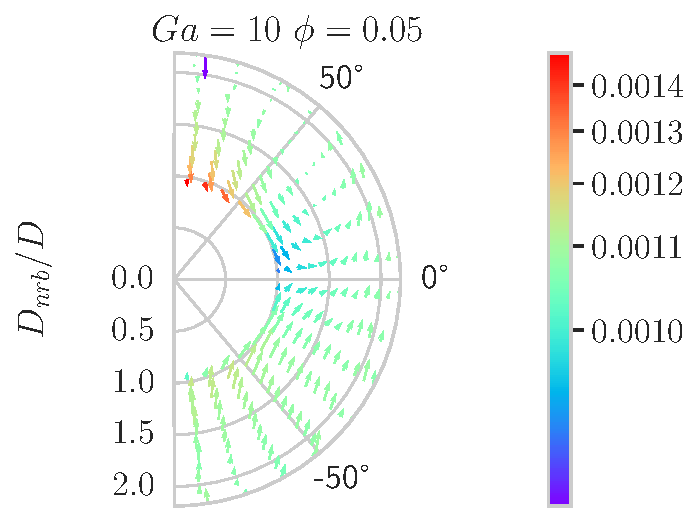
\includegraphics[height=0.2\textwidth]{image/Dim_3/fDrop/Dmin_Theta_ed_nbr_Ga_10_PHI_0_05.pdf}
    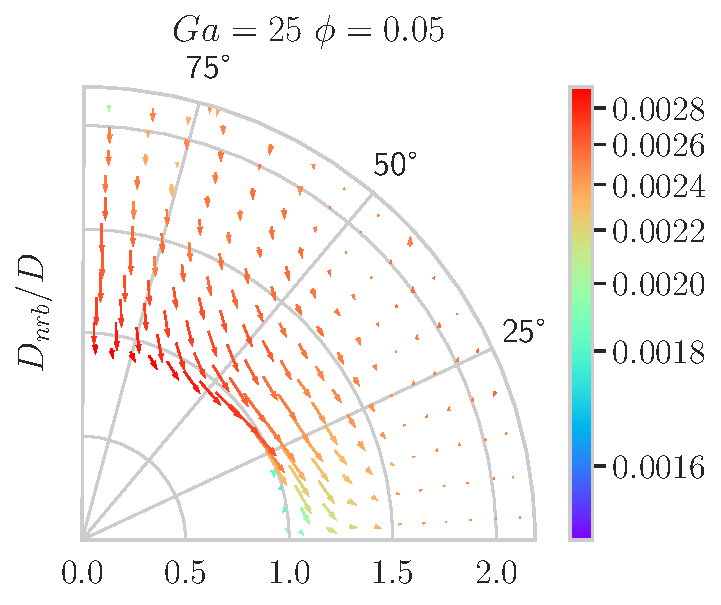
\includegraphics[height=0.2\textwidth]{image/Dim_3/fDrop/Dmin_Theta_ed_nbr_Ga_25_PHI_0_05.pdf}
    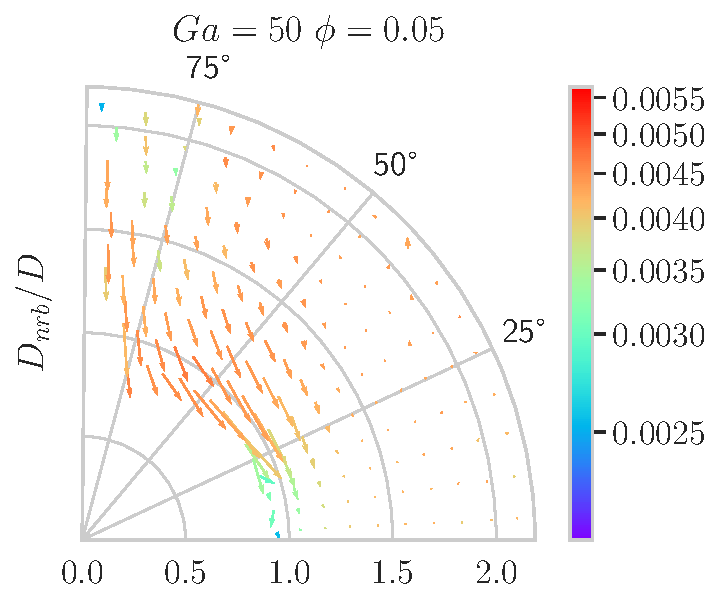
\includegraphics[height=0.2\textwidth]{image/Dim_3/fDrop/Dmin_Theta_ed_nbr_Ga_50_PHI_0_05.pdf}

    % 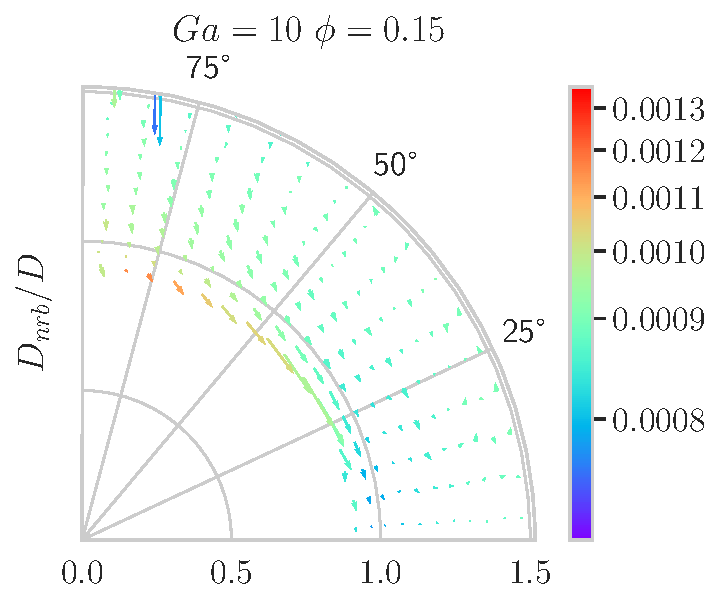
\includegraphics[height=0.2\textwidth]{image/Dim_3/fDrop/Dmin_Theta_ed_nbr_Ga_10_PHI_0_15.pdf}
    % 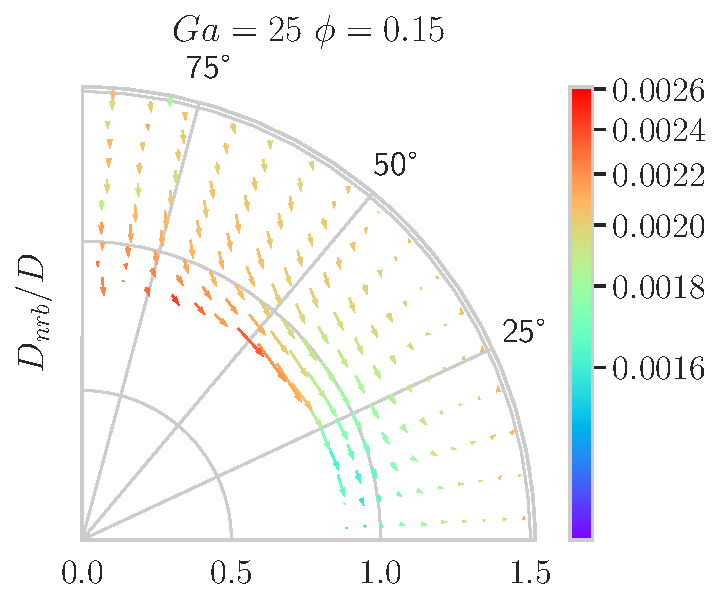
\includegraphics[height=0.2\textwidth]{image/Dim_3/fDrop/Dmin_Theta_ed_nbr_Ga_25_PHI_0_15.pdf}
    % 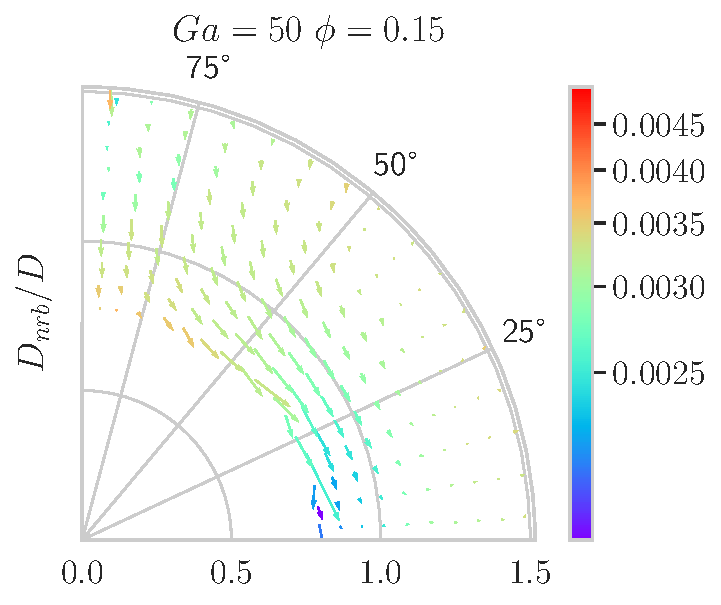
\includegraphics[height=0.2\textwidth]{image/Dim_3/fDrop/Dmin_Theta_ed_nbr_Ga_50_PHI_0_15.pdf}
    
    \caption{Nearest averaged velocity fields, $\nstavg{\textbf{u}}(\textbf{r})$ for different $Ga$ and $\phi$. 
    The color map scale the rate of dissipation of the nearest particle $\nstavg{\textbf{T}:\nablab\textbf{u}}$.}
  \end{figure}

\begin{itemize}
  \item If we assume that the collisions goes from the top to the sides, a dumping coefficient can be determinate. 
  \item Notice that the dissipation arise a lot before close contact.
  \item Thus, defining a collision with thresholds distance seems naive for collisions kernels.   
\end{itemize}
\end{frame}


\begin{frame}
  \frametitle{Microscopic representation of the particle pressure}

  \begin{figure}
    
    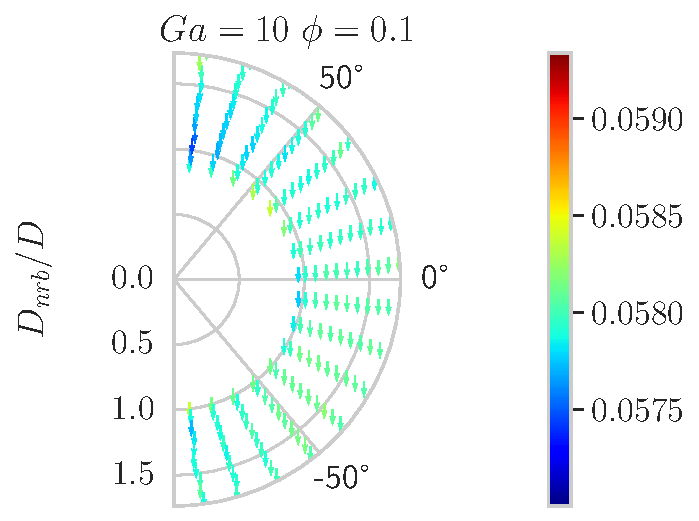
\includegraphics[height=0.2\textwidth]{image/Dim_3/fDrop/Dmin_Theta_Fh_nbr_Ga_10_PHI_0_1.pdf}
    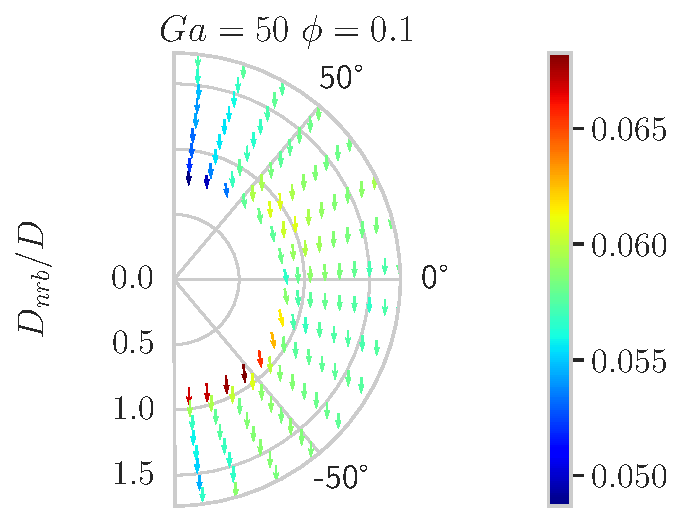
\includegraphics[height=0.2\textwidth]{image/Dim_3/fDrop/Dmin_Theta_Fh_nbr_Ga_50_PHI_0_1.pdf}
    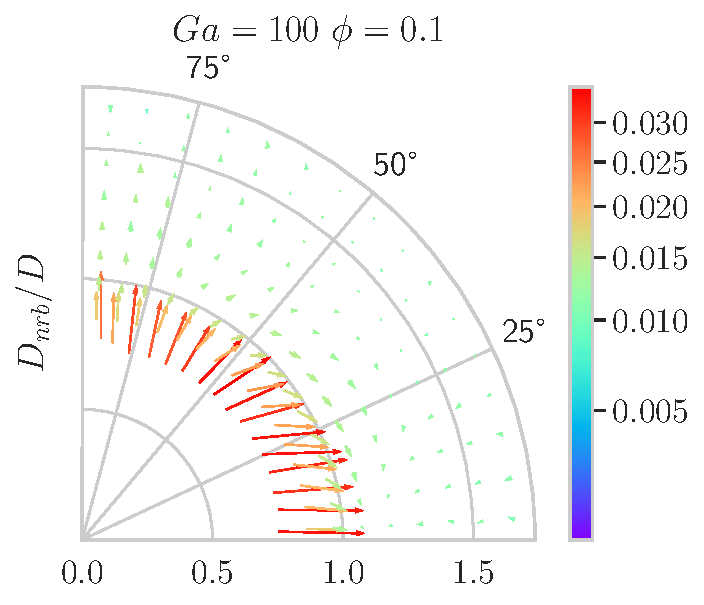
\includegraphics[height=0.2\textwidth]{image/Dim_3/fDrop/Dmin_Theta_Fh_nbr_Ga_100_PHI_0_1.pdf}

    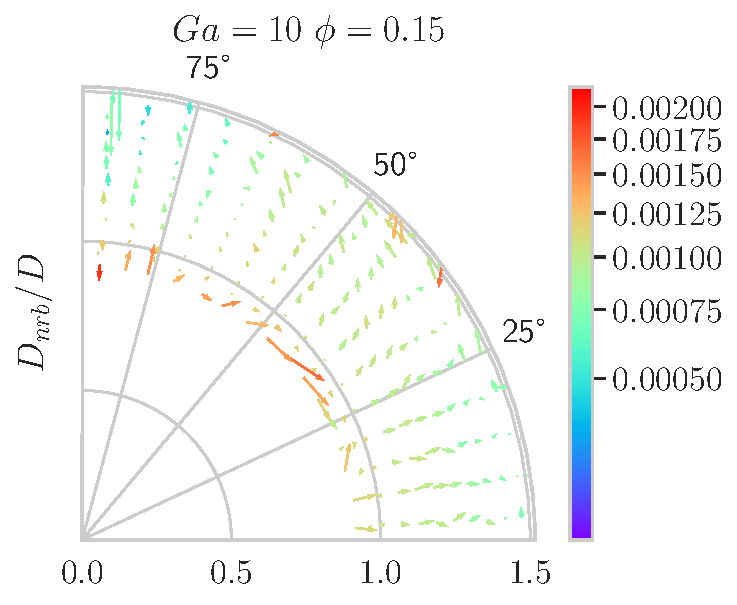
\includegraphics[height=0.2\textwidth]{image/Dim_3/fDrop/Dmin_Theta_Fh_nbr_Ga_10_PHI_0_15.pdf}
    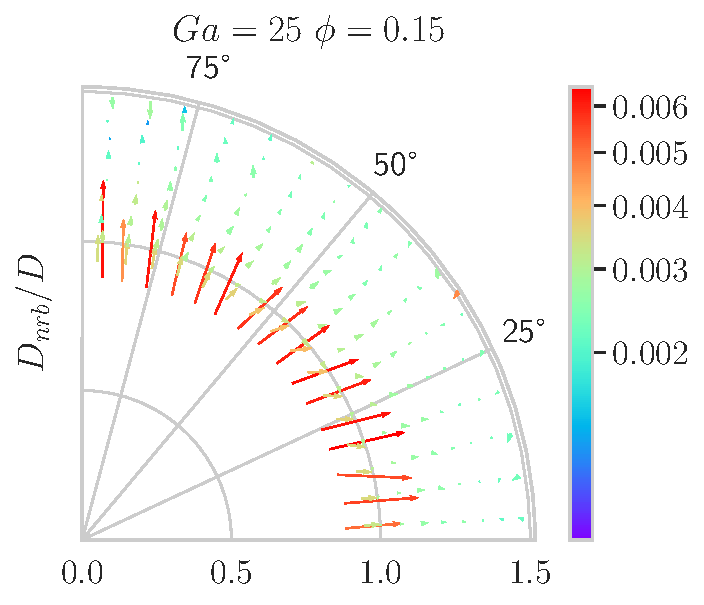
\includegraphics[height=0.2\textwidth]{image/Dim_3/fDrop/Dmin_Theta_Fh_nbr_Ga_25_PHI_0_15.pdf}
    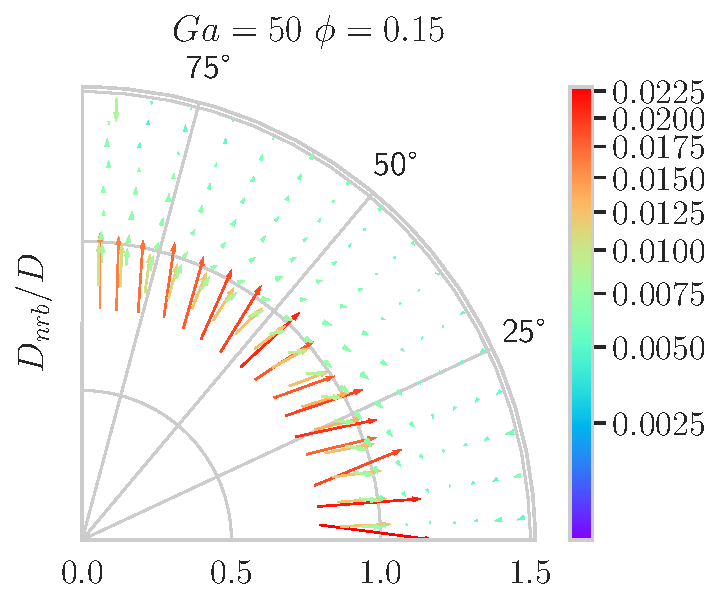
\includegraphics[height=0.2\textwidth]{image/Dim_3/fDrop/Dmin_Theta_Fh_nbr_Ga_50_PHI_0_15.pdf}
    
    \caption{Nearest averaged force fields, $\nstavg{\textbf{f}^2}(\textbf{r})$ for different $Ga$ and $\phi$. 
    The color map scales the magnitude of the force applied on the nearest particle $\nstavg{\textbf{f}^2}$.}
  \end{figure}

\begin{itemize}
  \item At low $Ga$, \textbf{f} is purely driven by the flow. 
  \item At higher $Ga$, \textbf{f} is directly correlated to the nearest particle. 
  \item Notice the higher magnitude interaction in the horizontal direction, which generate higher particle migration, and therefore oriented flows.
  \item This is a graphical representation of the particle stress.  
\end{itemize}
\end{frame}

\section{From microscopic representation to Macroscopic models}

\begin{frame}
  \frametitle{Microscopic to Macroscopic representation of the particule stress}
  \begin{columns}[c]
    \begin{column}{0.5\textwidth}
      \begin{figure}
    
        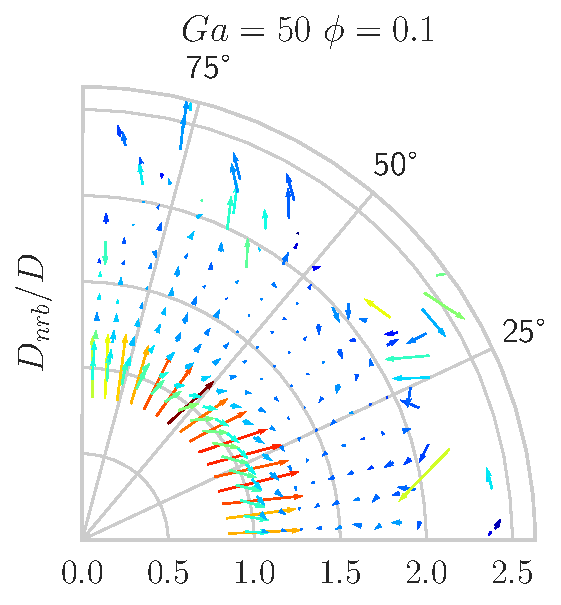
\includegraphics[height=0.6\textwidth]{image/Dim_3/fDrop/Dmin_Theta_Fh_Ga_50_PHI_0_1.pdf}
        
        \caption{Nearest averaged force fields, $\nstavg{\textbf{f}^2}(\textbf{r})$. 
        The color map scales the magnitude of the force applied on the nearest particle $\nstavg{\textbf{f}^2}$.}
      \end{figure}
    \end{column}
    \begin{column}{0.5\textwidth}
      The Pearson correlation between \textbf{r} and $\nstavg{\textbf{f}}$ turns out to be a stress tensor, such as, 
      \begin{equation*}
        \bm{\Sigma} = n \int \textbf{r} 
        \nstavg{\textbf{f}}(\textbf{r})
        P^2_{nst}(\textbf{r})
        d\textbf{r},
      \end{equation*}
      is the particule-fluid-particle stress. 
      For $Ga = 50$ and $\phi = 0.1$, we obtain, 
      \begin{equation*}
        \bm{\Sigma}^* = -\left[
          \begin{matrix}
            0.18 & 0 & 0 \\
            0 & 0.59 & 0 \\
            0 & 0 & 0.18 
          \end{matrix}
        \right]
      \end{equation*}
    \end{column}
  \end{columns}
\end{frame}

\begin{frame}
  \frametitle{Macroscopic representation of the particle stress}
The averaged interaction force through both phases can be written : 
\begin{equation*}
  \avg{\textbf{f}}
  =\avg{\textbf{f}}^{drag}
  + \nablab \cdot \bm{\Sigma}.
\end{equation*}. 
  \begin{figure}
    
    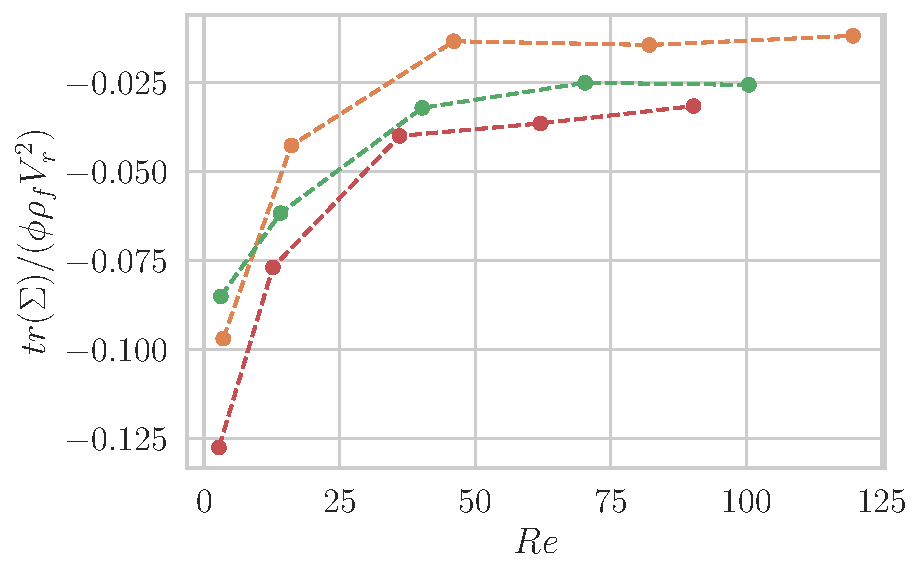
\includegraphics[height=0.15\textwidth]{image/Dim_3/fPA/PFP.pdf}
    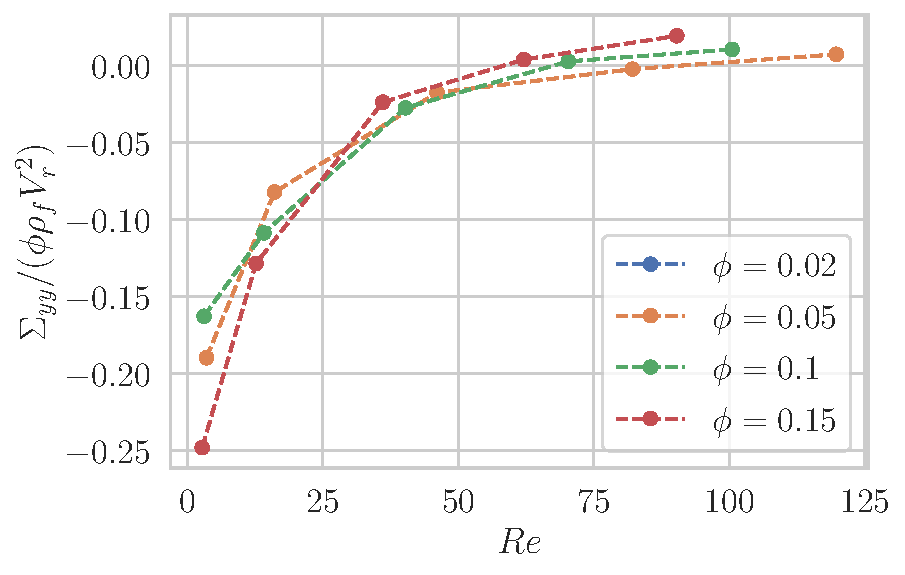
\includegraphics[height=0.15\textwidth]{image/Dim_3/fPA/PFP_y_y.pdf}
    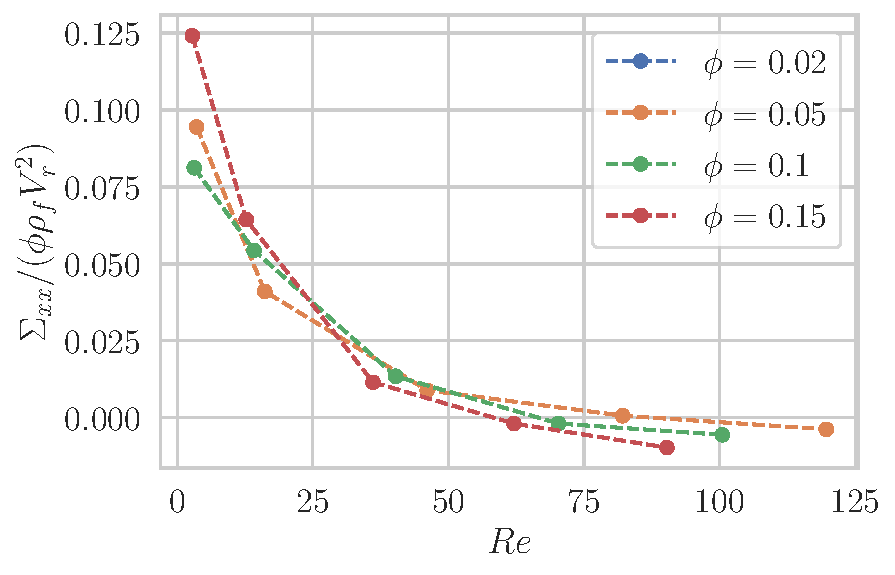
\includegraphics[height=0.15\textwidth]{image/Dim_3/fPA/PFP_x_x.pdf}
    
    \caption{Dimensionless particle stress, (left) on the vertical direction, (right) on the horizontal direction.}
  \end{figure}
\begin{itemize}
  \item The opposite sing between $\Sigma_{xx}$ and $\sigma_{yy}$ represent the contraction and spreading of the dispersed phase in each direction. 
\end{itemize}
\end{frame}

\begin{frame}
  \frametitle{Macroscopic representation of the relative nearest particular velocity fields}

  The source term of a property $q$ due to collision can be written \citep{rao2008introduction},
\begin{equation*}
  \avg{S}(\textbf{x}) = \int_{\textbf{r} \cdot \textbf{w} < 0} \left(q' - q\right)
  P^2(\mathcal{F}^1, \mathcal{F}^2)\textbf{r} \cdot \textbf{w} d\mathcal{F}^2 d\mathcal{F}^1 / d\textbf{x}^1
\end{equation*}
Beside, from \citet{zhang2021ensemble},
\begin{equation*}
  \avg{q}(\textbf{x}) = \int \nstavg{q}(\textbf{x},\textbf{y})P_{nst}(\textbf{y}|\textbf{x})d\textbf{y}
\end{equation*}
Beside, $P^2(\textbf{x}, \textbf{y}) = \frac{P_{nst}(\textbf{y}|\textbf{x})  n(\textbf{x})}{h_2(\textbf{x},\textbf{y})} $
\end{frame}
\begin{frame}
  \frametitle{Macroscopic representation of the relative nearest particular velocity fields}

  The source term can be rewritten as, 
  \begin{equation*}
    \avg{S}(\textbf{x}) =\textbf{I} : \int_{\textbf{r} \cdot \textbf{w} < 0} 
    \textbf{r} \nstavg{\left(q' - q\right) \textbf{w}}
    P_{nst}(\mathcal{F}^2| \mathcal{F}^1) d\mathcal{F}^2 d\mathcal{F}^1 / d\textbf{x}^1
  \end{equation*}
  Therefore the source term correspond to the Pearson correlation of the nearest particle relative velocities with its distance \textbf{r}. 
\end{frame}

\begin{frame}
  \frametitle{ Macroscopic representation of the nearest particule velocity fields}
  \begin{columns}[c]
    \begin{column}{0.5\textwidth}
      \begin{figure}
    
        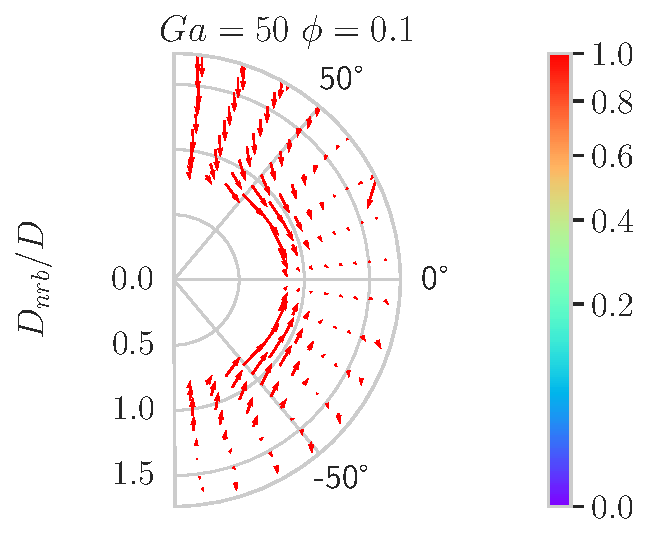
\includegraphics[height=0.6\textwidth]{image/Dim_3/fDrop/Dmin_Theta_U_rel_Ga_50_PHI_0_1.pdf}
        
        \caption{Nearest averaged relative velocity fields, $\nstavg{\textbf{w}}(\textbf{r})$. }
      \end{figure}
    \end{column}
    \begin{column}{0.5\textwidth}
      If $q=1$, the source term $S$ is the Pearson correlation between \textbf{r} and $\nstavg{\textbf{w}}$ and reads as,
      \begin{equation*}
        \overline{\overline{\textbf{U}}} = n \int \textbf{r} 
        \nstavg{\textbf{w}}(\textbf{r})
        P^2_{nst}(\textbf{r})
        d\textbf{r}
      \end{equation*}
      For $Ga = 50$ and $\phi = 0.1$, we obtain, 
      \begin{equation*}
        \overline{\overline{\textbf{U}}} = \left[
          \begin{matrix}
            4.6 & 0.6  & 0.2 \\
             0 & -9.5 & 0.1 \\
             0 & 0.2 & 4.7
          \end{matrix}
        \right]\cdot 10^{-3}.
      \end{equation*}
      \begin{itemize}
        \item Notice that $\textbf{r} \cdot \overline{\overline{\textbf{U}}}$ reconstruct the velocity field. 
      \end{itemize}
    \end{column}
  \end{columns}
\end{frame}


\section{Conclusion and discussion}
\begin{frame}
  \frametitle{General remarks and conclusion}

  \begin{itemize}
    \item The relative velocity, and forces are as we could see, directly correlated to the relative position and \textit{Galileo} number and volume fraction. 
    \item It is possible to create \textbf{Macroscopic} quantities, by carrying out the correlation between relative \textbf{Microscopic} position and the quantity of interest (as it has been shown with the particle stress). 
  \end{itemize}
  Future projects :   
  \begin{itemize}
    \item Derive a damping model for droplets interaction.
    \item Merge a film drainage model together with a detailed interaction function taking in account the angle of contact.
  \end{itemize}

\end{frame}

\begin{frame}[t]
  \frametitle{References}
  \bibliography{Bib/bib_bulles.bib}
\end{frame}
  
% \backmatter

\end{document}
